\chapter{Key Manager: Single Point of Failure}
\label{chap:key_manager}

In Chapter~\ref{chap:mgkmp}, we described a number of issues related to the MGKMP, without going deeper or proposing solutions. One more issue concerns the Key Managar (KM). For the latter, we decided we would be working more in depth on it, and propose a solution to solve the problem. This Chapter represent the internship's main mission, which led to the article publication.

\section{Problem description}
\label{sec:km_problem}

The whole architecture of the proposed solution above lays on one central component: the Key Manager. This vital component is to handle on its own the complete key management infrastructure and all the processes defined in the protocol, such as the rekeying process or key generation. Since we are considering a multi-group scheme, each group is handled by a Key Manager.

The Key Manager has to permanently satisfy the three main security properties: Confidentiality, Integrity and Availability (CIA). Any failure or the compromising of this machine will systematically jeopardise the whole security infrastructure of the group. A security breach of the KM can have devastating consequences, leading to the leak of the stored encryption keys used by respective group fellows.

A typical scenario is when the KM is down. This could be due to some malfunctioning in the system, or even a cyber-attack like a DDoS attack, or just result from some overload submitted to the KM, since it coordinates all nodes in the network. It could also occur upon an incident like a blaze in a datacenter \cite{malwarebytes}. In this situation, no rekeying process is going to be possible, as this operation is on the KM’s responsibility. Therefore if a compromised node is detected, either by neighbouring nodes or by a third party defense system like an IDS, it won’t be possible to have it evicted from the group. It wouldn’t be possible to have the group tided up neither. Basically, whatever device has detected the compromising, it would automatically report it to the KM in order to have it settled. However, since the KM is down, this eviction request will never be treated, and the cleaning up operation will never be carried out. Moreover, as long as the KM remains down, the compromised node will remain a member of the group having all group’s communication it’s allowed to compromised. Furthermore, the node not being evicted once it’s uncovered, it can spread into the network compromising all group related keys it hasn’t yet in its inventory.

\begin{figure}[htbp]
	\centerline{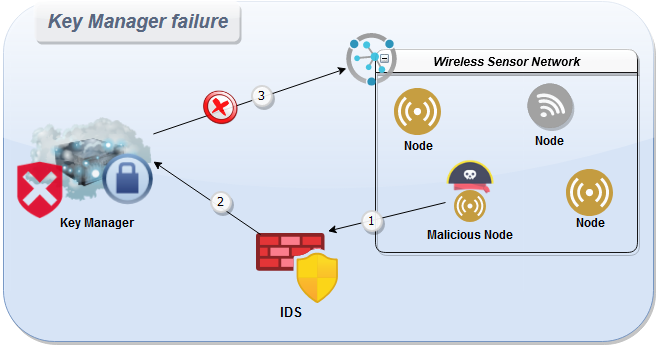
\includegraphics[scale=0.55]{figures/mgkmp/failure.png}}
	\caption{Key Manager failure scenario}
	\label{fig:km_failure}
\end{figure}

One would want to say that if we add some redundancy to the KM, that would solve the problem. If the main KM is down, then we have some backup clones to take over until the main one is on track again. Nevertheless, this isn’t necessarily guaranteed, because availability isn’t the only security requirement to satisfy as mentioned above. To illustrate this, we can imagine an interference in the communications from and to the KM. A malicious node or a third party attacker can spoof the KM’s identity and hence, conduct a Man in the Middle (MITM) attack. If the KM is compromised, then so are all operations it is carrying out and the infrastructure as a whole would be rotten to the core. Even if the communications are encrypted, the attacker can still tamper with a rekeying process upon a node’s leave. Actually, if the attacker has access to the leaving node’s keys, then he can forge rekying messages with the old revoked keys. That way it would be as the whole rekeying operation hasn’t took place, and the leaving node will have a theoretically unauthorised access to so many communications, making them all compromised. An attacker acting like a proxy for the KM can also intercept messages for a joining node. But as a pre-secure channel should be established between the KM and the new node, the way he can compromise these messages depends on how this channel is implemented.

This attack is a bit more difficult than the previous to mount though, since the attacker has to manipulate data (eg. the ARP table) for every node and other entity that might be in interaction with the KM. Unless the KM is placed behind a single component, such as a Firewall, then the attack difficulty would depend on the resilience of the latter.

\begin{figure}[htbp]
	\centerline{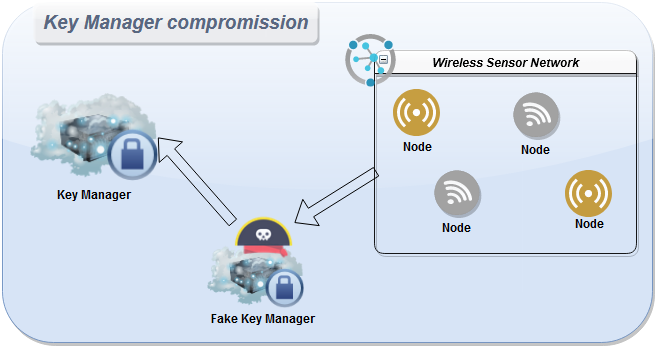
\includegraphics[scale=0.55]{figures/mgkmp/comprom.png}}
	\caption{Key Manager compromising scenario}
	\label{fig:km_mitm}
\end{figure}

To sum up, we have two main problems concerning this architecture making out of the KM a single point of failure. The first one concerns the load imposed over the KM. It has to coordinate every node from groups and subgroups. Every join or leave operation is validated by the KM, and the consequent rekeying operations are also handled by it. In the original design, we already assume that the KM is powerful and robust. But such performance assumptions can be costy, and still, it remains a system with its own physical limits like any other system. All this makes the KM a \textbf{\textit{single point of charge}}. Second, we also make the assumption that the KM is trustworthy. The fact that all network membership evolution have to be validated by the KM, and the rekeying process is entirely handled by it as well, gives it a large base of trust. The MITM attack described above shows how critical this trust can be. This makes the KM a \textbf{\textit{single point of trust}}. A way to mitigate these risks, is to design a decentralised architecture with a distributed base of trust and a distributed load of charge.

\section{Blockchain-based scheme}

Kandi et al. \cite{kandi_lightweight_nodate} suggested a solution based on the Blockchain technology as explained previously (see Chapter~\ref{chap:litterature}). This solution however might end up too costy for IoT networks. One one side, the Blockchain implies that all nodes, regardless of their storage capacity, will have to store the ledger, which will definitely cause a significant additional storage overhead. The more traffic we have (nodes joining and leaving), the more blocks have to be added. This makes the storage overhead, in addition to its height, dynamic and of an unpredictable growth. Moreover, these transactions will introduce a consequent network traffic. Hence, an increase in bandwidth consumption and drainage of node’s already-constrained resources. Besides the performance hindering, a hacker can see in this an opportunity to conduct a parallel DoS attack. By maliciously interfering with the network traffic, one can instigate false join and leave requests, which will be translated into appended blocks to the ledger. Abusing this kind of interference might consume the total node’s storage capacity. On the other side, each block append to the ledger requires a computational effort, a Proof of Work. PoW operations or even PoS operations in the Blockchain aren’t the most trivial to compute. They require a certain minimum threshold of computational power, and the way the Blockchain technology was designed in the first place, tend to have such threshold as high as possible, which is exactly what we want to avoid. Even with some lightweight versions of the Blockchain, it doesn’t resolve entirely the problem and it may very well add further problems. Those lightweight versions are actually based on constraint-reduced PoW or PoS. However, this can open the door for some security risks since transactions would be easier to validate, and so the vote process will be more accessible. Hence, malicious nodes will be more likely to conduct veiled activities, and we’re not even sure if the computational capacity problem is solved.

\section{Election-based scheme}
\label{sec:election-based-scheme}

Another strategy for distributed charge and trust for the Key Manager, is to have an election-based scheme, where any node can be the KM. This way, we mitigate the risk of single point of failure present in the original design on one hand. And on the other hand, we don’t necessarily have all nodes assuming the costy role of a KM like in a Blockchain-based scheme. The main idea is that one node among the group will assume the responsibility of a KM (which is already possible in the centralised version). This node has been chosen and approved by the others. This choice is based on some node-related technical criteria, which make it eligible for this role. In case the KM down or compromised, any other eligible node can take over. A KM can also choose, if the situation allows and requires it, to hand over its responsibilities in case it is or will be suffocating. The KM still uniquely assumes the responsibility of the key generation process during a rekeying operation, but it can share the burden of newly generated keys distribution with the others. In this scheme, key generation has also been improved and optimised for less energy drainage. In addition to the role of a KM, we also define a deputy, which is the privileged node to take over if the KM is, for some reason, deemed to step down. This deputy has also a monitoring role over the KM.

\begin{figure}[htbp]
	\centerline{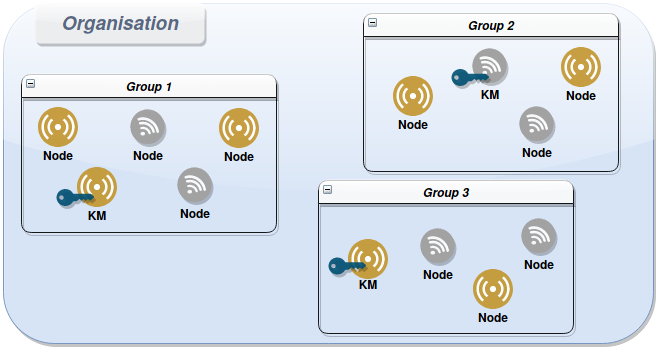
\includegraphics[scale=0.50]{figures/organisation.png}}
	\caption{Election-based scheme architecture}
	\label{fig}
\end{figure}

In Section 1.1.2, we discussed several Cluster Head (CH) selection algorithms. However, these algorithms were mostly designed to address network routing and data exchange problems, such as LEACH (Low-Energy Adaptive Clustering Hierarchy) \cite{heinzelman_energy-efcient_2000} and related extensions \cite{al-baz_new_2018, kang_distance_2012}. Other algorithms for CH selection seeking to optimise energy load-balancing were  proposed in \cite{behera_residual_2019, jia_dynamic_2016}. These algorithms utilizes node’s energy capabilities to balance probabilities for CH selection among other cluster nodes. But all these studies aim to optimise energy performances with no regard to security. They were basically developed to save radio transmission overhead, thereby they deal with network and data routing oriented problems. However, our interest for this scheme is foremost driven by our need to solve the Key Management problem for group communication and provide a decentralised model for it. Moreover, the CH election in previous works is based on energy, communication and networking related criteria. Besides, they mainly consider homogeneous environments in which CH are to communicate with a fixed Base Station (BS) for application reasons. Hence, the described models are not necessarily adapted for use as a security oriented scheme (cryptographic key management in our case) for heterogeneous IoT networks. In our use case, we tend more to think over the architecture from a security point of view. The main security criterion the CH must satisfy is availability. We are not using the CH a as relay between nodes and some BS. We are rather building a security infrastructure to manage cryptographic keys in order to secure both group and device-to-device communications between different nodes. When rethinking the election-based scheme from this prospective, we actually end up with many additional constraints than those already considered.

\begin{figure}[htbp]
	\centerline{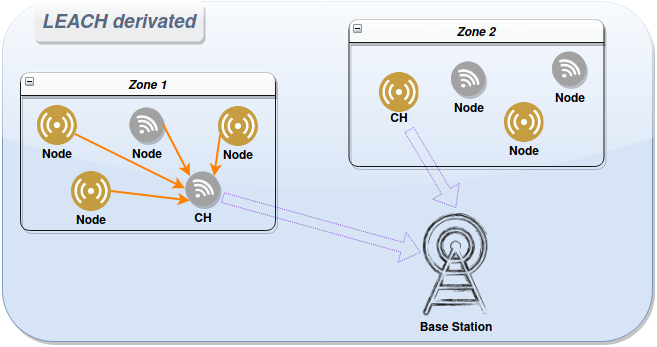
\includegraphics[scale=0.50]{figures/LEACH.png}}
	\caption{Overview of LEACH-based architecture}
	\label{fig}
\end{figure}

In this section, we propose a new complete election-based scheme adapted for Key Management in multi-group IoT networks. The point is to successfully define a decentralised election-based infrastructure for Key Management which (i) solves the problem of KM single point of failure, (ii) satisfies the heterogeneous and energy-constraint nature of IoT networks, (iii) considers the main objectives we target from a security point of view, and (iv) tries to inherit as possible the features offered by previous work (even thought not all of those are needed for our use case).
In the very first basic approach, the idea was to have one unique component that handles the Key Management, where came the problem of single point of failure from. In the first attempt to solve the problem, the Blockchain technology was considered, where the energy consumption problem came from. So we basically went from having one single node doing this heavy important task in the first case, to a state where all nodes are assuming this role regardless of their capabilities in the second case. The approach we would like to propose tries to combine both previously mentioned approaches in order to suggest something in between. The advantage of the election-based approach is that it have one particularly capable node acting as KM (the first approach likewise) while actually allowing any node in the network to take part (the second approach likewise). The fact that this node will be elected and validated guarantees the reliability of the KM from both security and performance point of view. Therefore, the architecture should support decentralised decision making, and thus enhance failure management. As for the KM election, it should take into consideration security concerns through consensus-based trust. Finally, to maintain scalability and IoT performance requirements, the architecture must be flexible and involve minimum vote processes and communication overhead.

\subsection{Technical eligibility criteria}

Basically, any node can be the KM and that’s the basis to have a distributed system. However, those can be heavy and expensive responsibilities to assume, which require minimum capacities in networking, storage and processing. Otherwise the node could be merely qualified as single point of failure by default. To ensure that a candidate node will be up to it when qualifying for KM, we define two new functions: Processing Capacity Evaluation Function (PCEF) and Networking Capacity Evaluation Function (NCEF). Those two new functions will be aggregated with the already defined Storage Capacity Evaluation Function (SCEF) as an input for the Capacity Evaluation Function (CEF). The latter's output is what gives us the bigger picture about the node’s real technical capabilities and qualification for the KM’s assignments. The output of the CEF is a score, which has to be above a minimum threshold for a node to be eligible for the role of the KM. The final score value shall be correlated with the node’s energetic capacities as well. This settled, we ensure that an elected node for KM is indeed technically and energetically reliable.

The CEF score should be an average value totally blinding regarding the input values. For this purpose, the input values could, eventually, be aggregated with a salt to add some noise. There are two main reasons why the CEF’s output is a single dark value. The first reason is saving network bandwidth and energy. In this form, a node will be just broadcasting a number, instead of a long message detailing its capacities. Besides, this increases accuracy when providing a reference scale for decision making (voting). The second one is security related. One is never sure whether a pre-compromised node is present in the group like a Trojan horse, or an outsider attacker is somehow eavesdropping on the group communications. Therefore, it’s more secure if the CEF score doesn’t leak any data about a node’s real capabilities in networking, storage and processing. The acquisition of such information can be used to mount other specific attacks, and so very harmful. A typical example, is side channel attacks in cryptanalysis. Knowledge of some physical properties of a device can significantly increase the efficiency of these category of attacks, in a context where cryptographic choices are critical (see Section 3.4).

\begin{figure}[htbp]
	\centerline{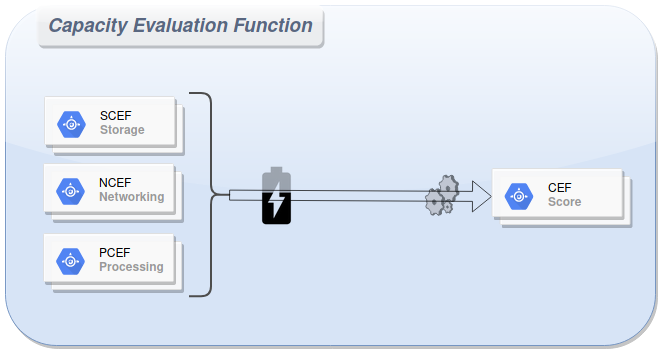
\includegraphics[scale=0.50]{figures/cef.png}}
	\caption{Capacity Evaluation Function score}
	\label{fig}
\end{figure}

\subsubsection{Technical description of CEF score}

The CEF score is computed based upon three inputs SCEF, PCEF and NCEF correlated with an energy score.

First of all, we start with the SCEF since it’s already at our disposal. The KM, as its name suggests, will have to manage keys. Among other things, it stores all cryptographic keys used to secure communications within the group, as each group has an independent KM, and exchanges with other groups. The larger the group is, the more related keys the KM will have to manage. Thus, the KM must have some some storage capabilities, especially if we want to preserve the scalability which can involve numerous group fellows. The SCEF was defined in \cite{kandi_versatile_2020} by:

\begin{equation}\label{eq1}
	c_k = pm \; .\; \frac{sc_k}{ks}
\end{equation}

where
\begin{math}
	\left\{
	\begin{array}{l}
		s_k: storage\; capacity\; of\; a\; node\; u_k\\
		sc_k: storage\; capability\; of\; a\; node\; u_k\\
		pm: usable\; percentage\; of\; memory\; by\; protocol\\
		ks: size\; of\; a\; key
	\end{array}
	\right.
\end{math}\\

For conformity issues, we bring slight edit to the notations above, thus redefining the SCEF as:

\begin{equation}\label{eq2}
	s_k = pm \; .\; \frac{sc_k}{ks}
\end{equation}

\begin{math}
s_k:\; storage\; capacity\; of\; a\; node\; u_k
\end{math}

The rest of notations are maintained.

The next step is the definition of PCEF. The PCEF is a function we introduce in order to assess the processing capacities of the node, a potential KM candidate. Actually, all group related keys are exclusively generated by the KM. But a key generation involves the execution of cryptographic functions, which are by default expensive in terms of processing. As discussed in Section~\ref{sec:mgkmp_liabilities}, lowering the standards of cryptographic systems implementation may degrade its reliability. Thereby, enough processing capacities are crucial to maintain a high resilience level of the protocol. In Section 5.1.1 of \cite{kandi_versatile_2020} related to the theoretical analysis of the overheads of the KM, we cite:

\begin{quote}
	Property 2: Calculation overhead on the KM is proportional to the sum $p+m_j$.
\end{quote}

Based upon this property, we define the PCEF score as follow:
\begin{equation}\label{eq2}
	p_k = pp \; .\; \frac{cc_k}{cs \; .\; \left( p + m_j \right)}
\end{equation}

where
\begin{math}
	\left\{
	\begin{array}{l}
		p_k: processing\; capacity\; of\; a\; node\; u_k\\
		cc_k: computation\; capability\; of\; a\; nod\;e u_k\\
		pp: usable\; percentage\; of\; processor\; by\; protocol\\
		cs: overhead\; of\; crypto\; system\\
		p: number\; of\; subgroups\; of\; the\; group\; G\\
		m_j: number\; of\; nodes\; in\; subgroup\; S_j
	\end{array}
	\right.
\end{math}\\

The above definition of pk takes very well into consideration the fact that the KM will handle exchange security between other groups and his own, during different rekeying operations, according to the rekeying procedure defined in MGKMP. The function considers the percentage of processing the protocol can use. This means that nodes which processing units are perfectly designed to only handle their application related tasks, such as some wireless sensors, won’t be very favorable as KM candidate. The computation capability $cc$ is a static value based on physical characteristics of a device (eg. the processing unit’s frequency in Mhz).

The last of the three capacity criteria to consider is the NCEF. Rekeying operations, as defined in MGKMP, involve big time communication overhead for the KM, from joining messages to leaving messages. Besides, theses messages are transmitted in all possible fashions: unicast, multicast or broadcast. Moreover, for a newly joining node, the first communication channel is to be established with the KM in order to proceed with the join (see Section~\ref{subsec:node_join}). This channel has to be robust from a networking point of view, and shall not be hindered by low networking capabilities. As mentioned, rekeying operations might require the KM communicating with other groups, eventually physically far distanced, which even highlights further the importance of communication range and strength of the KM candidate. Even if the node is selected as supplicant KM, it will have the task of monitoring the main KM, which involves way a lot of networking. The deputy KM has to be ready to assume functions of an active KM at anytime anyway. In Section 5.1.1 of \cite{kandi_versatile_2020} related to the theoretical analysis of the KM's overheads, we cite:

\begin{quote}
	Property 1: Communication overhead on the KM is proportional to the sum $p+m_j$.
\end{quote}

Based upon this property, we define the NCEF score as follow:

\begin{equation}\label{eq3}
	n_k = bw_k \; .\; \frac{rr_k}{\left( p + m_j \right) \; .\; \max\left( ms \right)}
\end{equation}

where
\begin{math}
	\left\{
	\begin{array}{l}
		n_k: networking\; capacity\; of\; a\; node\; u_k\\
		bw_k: bandwidth\; of\; u_k\; usable\; by\; the\; protocol\\
		rr_k: radio\; range\; of\; u_k\\
		ms: size\; of\; a\; message\\
		p: number\; of\; subgroups\; of\; the\; group\; G\\
		m_j: number\; of\; nodes\; in\; subgroup\; S_j
	\end{array}
	\right.
\end{math}\\

Once again, the KM may be dealing with inter-group communications during rekeying operations, as defined in MGKMP. Therefore, the forehead definition of $n_k$ takes the radio range of $u_k$ into consideration, for practical usability concerns.

Following the three main technical criteria, one extra criterion is considered to ensure energy reliability of the KM. Both processing and foremost networking are energetically expensive. The energy correlation value is made up to adjust the final CEF score to favor the most green of nodes. It is defined as follow:

\begin{equation}\label{eq4}
	e_k = \frac{re_k}{ed_k \; .\; pu_k}
\end{equation}

where
\begin{math}
	\left\{
	\begin{array}{l}
		e_k: energy\; attribute\; of\; a\; node\; u_k\\
		re_k: residual\; energy\; of\; a\; node\; u_k\\
		ed_k: energy\; drainage\; of\; u_k\\
		pu_k: percentage\; of\; processor\; in\; use\; for\; u_k
	\end{array}
	\right.
\end{math}\\

The function considers only remaining energy of the device by the time the election process is kicked off, then it’s a dynamic value that evolves (mostly decreases) overtime. The device’s total energy is not relevant. Energy drainage of $u_k$ is actually a static value based on physical characteristics of a device. It could for instance the energy consumed in $J.s^{-1}$ during transmission or processing.

With all input values settled, we can finally compute the final CEF score as follow:

\begin{equation}\label{eq5}
	c_k = e_k \; .\; \left( w_s s_k + w_n n_k +  w_p p_k \right)
\end{equation}

where
\begin{math}
	\left\{
	\begin{array}{l}
		c_k: capacity\; score\; of\; a\; node\; u_k\\
		w_s: storage\; capacity\; weight\\
		w_n: networking\; capacity\; weight\\
		w_p: processing\; capacity\; weight
	\end{array}
	\right.
\end{math}\\

It’s this very ck which will serve as score to assess the overall capacity of a node $u_k$, and serve as basis for the election process. Weight correlation values are first determined through simulations and experiments. Their values remain static afterwards, thus to limit computation overhead of the CEF and increase the protocol’s efficiency.

\subsubsection{The Run Threshold}

We introduce the election run threshold, dubbed $rt$, as a static or dynamic value. In order for a node to run in an election, the node’s CEF score has to be above this threshold. There is no formula for the value of $rt$. Since it depends very much on the used hardware and the use case application, it actually has be determined later on by simulations and experiments during the implementation of the protocol. Nevertheless, we consider by default that it’s set to $rt=0$. This threshold actually limits the number of participating nodes as candidates during the election. Therefore, it decreases the overall bandwidth consumption during the election, and improves the votes accuracy.

\subsection{Operational Mode}

This Section mostly describes the solution's algorithmic behavior. It defines different newly introduced entities and describes their roles as well.

\subsubsection{The role of deputy KM}

In addition to the active KM, we introduce a supplicant KM, also dubbed as deputy KM. In the following, the main CH will be referred as main KM, active KM or simply the KM. It has two main functionalities. First, it’s the node to take over the active KM when needed. This can be upon the compromise or breakdown of the latter, or just for rotation. This need to have a well designated node ready to immediately take over is necessary to prevent a void in the head of the group. Such void in leadership is, just like in real life, a huge security vulnerability which leaves all the group’s communications at risk. Second, the deputy KM can serve as a monitoring device for the active one. It would check over it regularly to verify it’s neither inactive nor compromised. This check over message could be a simple ping message, in case we just want to verify the main KM’s availability. In case we want the check over to include both availability and integrity of the main KM, then the supplicant can just send a challenge to the KM. If the KM doesn’t answer at all over a certain time lapse, then it’s down. If the KM replies with a wrong answer, then it’s compromised. In both situations, the deputy KM knows it must take matters into its own hands. Since the beginning of the protocol’s definition, we often assume the presence of a security component in the network, in charge of monitoring availability and integrity of all network’s nodes altogether. With this solution, we actually (i) make the protocol less dependant on external entities and ready-to-take assumptions, since the monitoring process is thereby partially internalised within the protocol. Thus, it makes the protocol more resilient. We also (ii) manage to decentralise the KM’s failure detection and recovery, since we have one deputy KM per group to take care of it. Thus, it makes the protocol more scalable.

\begin{figure}[htbp]
	\centerline{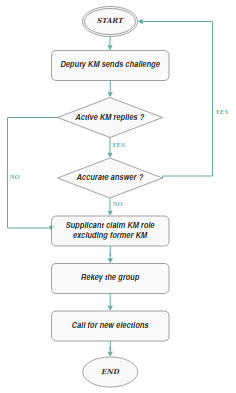
\includegraphics[scale=0.72]{figures/recovery_workflow.png}}
	\caption{Failure recovery workflow}
	\label{fig:recovery_workflow}
\end{figure}

\subsubsection{Election mutual exclusion and roles definition}

The protocol’s design assumes that a node can belong to two distinct groups in the same time. Basically, a node cannot be the KM for more than one group. Nodes dispose of a binary parameter $elected$, by default set to $False$. If a node gets elected in the context of any group it belongs to, this parameter is switched to $True$. If a node $n_i$ is affected to the two distinct groups $G_1$ and $G_2$, while also been elected KM for $G_1$, then it definitely is not and will not be the KM for $G_2$. If some election takes place in the context of $G_2$, $n_i$ will have its parameter elected already set to $True$. Hence, it just won’t broadcast its CEF score, and so won’t be promoted as a potential candidate. But this restriction doesn’t prevent the node from participating in the voting process.

In case a node other than the KM is compromised, the KM has the charge of the rekeying operation, as originally defined in MGKMP. Upon a node’s join or leave, the procedure remains the same as well. However, if it’s the KM itself which is detected as compromised or flooded with a huge charge of tasks, then a failure recovery process is instigated. When in place, the detection is done by the deputy KM.

To enhance the scheme’s performance and strengthen its decentralised side, we introduce two operational optimisations regarding tasks mainly handled by the KM. One concerns the key share during rekeying process, while the other is more about its very own generation. During a rekeying operation, the KM is responsible for new keys generation as mentioned. These new keys shall be communicated to the concerned group members. For this, the KM doesn’t necessarily have to deliver it to every node one by one. Some fellow members might already have pre-established communication channels between them, encrypted with keys known to only both of them. To save its energy and bandwidth, the KM might rely on other fellows, having low energy-consuming tasks, to relay the information in a peers-seeders fashion. Besides, upon a new node’s join, the KM doesn’t necessarily have to generate new keys for the rekeying operation. It could actually make use of prefix encryption and generate derived keys from the old ones. Nodes detaining the old keys, those are group fellows, are able to guess the new ones. But the joining node, receiving the new keys, won’t be able to climb up to the old ones, which satisfies the forward secrecy requirement. This however is applicable only to node join operation. By definition, this prefix encryption enhancement cannot work out for node leave or eviction operations.

\subsubsection{Inter-group communications management}

In the reviewed literature (Section~\ref{subsec:ch}), election-based schemes assume a CH for each group. Since proposed solutions are aimed at addressing routing problems, groups were not supposed to communicate between each other. For instance, each group has its own KM, and the latter shall mind only his groups internal business. Therefore, they manage only intra-group communication issues. However, the MGKMP leaves the door open for inter-group communications. In the original centralized scheme, the problem wasn’t even to worry about since we have one central KM for the whole network. In order to solve this issue, our solution suggest that every KM within the network is capable of operating on the inter-group level, and it’s the situation that determines which one in particular to do it. The design of MGKMP assumes that nodes hold DEKs and KEKs to secure group communications on the service level. These keys are very important, because they’re used by nodes in order to enhance the protocol’s scalability and efficiency. Nevertheless, a group by definition is a unique combination of service(s). Hence, These mentioned keys actually involve communications on the inter-group level, which we will refer as the federal level. It’s right here where the limit of previously proposed works on CH schemes bring front another limitation: if we have a KM for every group, such is our case, which entity is responsible for tasks involving more than one group ? If we look deeper these so-called federal processes, they mainly interfere during rekeying operations, the KM’s main task. So basically, the renewing of these service related keys occurs in the aftermath of a group’s membership update (node’s join, leave or eviction). Therefore, we assume that it’s the KM for the concerned which will handle the whole task. It will take of renewing the group-related keys and all the other keys requiring renewing. Then, it will communicate these keys to the concerned groups if necessary. This way, any locally elected KM can actually be the federal KM, and may assume these double role whenever the situation requires it. Handling two positions simultaneously and for a short time slot makes this solution efficient. Allowing all so-called local KMs to do it makes the inter-group key management decentralised, and thus, the solution scalable and compatible with heterogeneous networks.

\subsection{Election process}

This section describes the election process. It defines notations related to the operation, and enumerate its different steps.

\subsubsection{Group Key}

Since the election takes place in the context of a one particular group, the election procedure detailed in the forthcoming paragraph would actually require broadcast operations within this group. These transmission should be encrypted on the group level. However, the MGKMP as defined do not introduce such key, probably because it’s not actually needed for its main purpose, rekeying operations. Groups were basically designed to be logical and completely transparent to the application. As for Key Management and rekeying processes, we can do with just service keys and subgroups keys, no need for group keys. Thus, in order to secure communications with in a group without limiting ourselves to subgroup constraints, we have one existing solution. Since a group is a unique combination  of services, we could secure the message by encrypting over with all relevant service keys. All nodes belonging to the group are, by definition, holders of necessary keys to decrypt the message. Nevertheless, this solution turns out to be very expensive in terms of processing. Therefore, we introduce in this section a Group Key. We denote $K_i$ the Group Key of the $i^{th}$ group, held by all group members. This assumption increases very slightly the storage overhead for nodes. But, it saves much more in the processing overhead, and thereby less energy consuming.

\subsubsection{Notations and messages glossary}

\begin{equation}\label{eq6}
	EM1: CH \Rightarrow G_i : \langle\; \varnothing\; \rangle_{K_i}
\end{equation}
a call for election broadcasted by either current KM or its deputy

\begin{equation}\label{eq7}
	EM2: u_k \Rightarrow G_i : \langle\; c_k\; \rangle_{K_i}
\end{equation}
CEF score broadcast by potential candidate

\begin{equation}\label{eq8}
	EM3: u_k \Rightarrow G_i : \langle\; m,\; n\; \rangle_{K_i}
\end{equation}
vote broadcast by elector node, where $u_m$ and $u_n$ are the voted KM and supplicant respectively

\begin{equation}\label{eq9}
	EM4: u_m \Rightarrow G_i : \langle\; \varnothing\; \rangle_{K_i}
\end{equation}
KM role claim broadcast

\begin{equation}\label{eq9}
	EM4_{bis}: u_n \Rightarrow G_i : \langle\; \varnothing\; \rangle_{K_i}
\end{equation}
supplicant role claim broadcast

\begin{figure}[htbp]
	\centerline{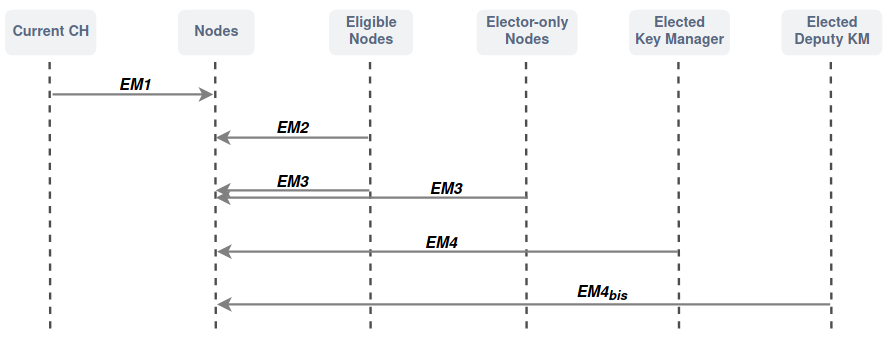
\includegraphics[scale=0.40]{figures/election_exchange.png}}
	\caption{Election process message exchange}
	\label{fig:election_msg_exchange}
\end{figure}

Fig.~\ref{fig:election_msg_exchange} demonstrates the assumed sender of each message. The timeline order of sending these messages goes from $EM1$ to $EM4$/$EM4_bis$. As shown in the figure, all message are actually broadcasted by their source nodes to the whole group.

\subsubsection{Election procedure}

The choice of the KM and eventually its deputy is based on an election procedure, during which nodes will vote for the most reliable KM. The procedure’s outcome must satisfies the election of a technically reliable and secure KM, while consuming the minimum of bandwidth.

\begin{figure}[htbp]
	\centerline{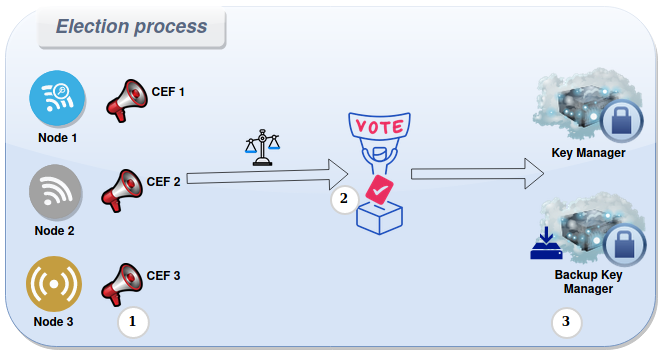
\includegraphics[scale=0.50]{figures/election.png}}
	\caption{Election procedure}
	\label{fig:election_proc}
\end{figure}

When an election trigger is pulled, the current CH, whether KM or supplicant, will instigate the election procedure. It first broadcasts the message $EM1$ to the relevant group. This message is a call group members for elections. Once group fellows receive this message, each potential candidates will update their CEF score. These nodes must definitely have their $elected$ parameter set to $False$. Nodes which $elected$ parameter is set to $True$, are deemed not to run and would skip this step. For each running node, if its updated CEF score is higher than the $rt$, it then braodcasts the message $EM2$ to group members. This message contains the updated CEF score and the identifier of its sending node, for others to benchmark to most reliable candidate. Followingly, nodes will receive different capacity scores from different candidates. Thereby, they dispose of a list of scores corresponding to group fellows, including their own if they’re candidates. Every node will benchmark scores in its list in order to choose the highest two. Then it will broadcast the message $EM3$, which contains identifiers of both chosen candidates for KM and supplicant roles respectively. Now every candidate node receiving this message will keep a count of which node received most votes. So theoretically, the count should be the same for every node, with the exact number of votes for the same couple of KM/supplicant, knowing who the ones are. However, due to the probabilistic aspect of networking and some nodes IoT-related liabilities, it doesn’t always work out perfectly as expected. That’s why we are keeping track of this count. If a candidate node sees that it has been elected for either role, it has to claim it. In case the node is elected as KM, it will broadcast the message $EM4$ to the group, which contains its identifier and useful coordinates. This message announces to the group that the sending node is the new KM. In case the node is elected as supplicant to the KM, it will broadcast the message $EM4_bis$ to the group, which contains its identifier. This message announces to the group that the sending node is the new deputy KM. Now this is concerning candidate nodes. For the rest of elector-only nodes, they actually go into a stall mode since sending message $EM3$. They don’t need to neither receive other nodes $EM3$ messages, nor keep track of the election progress. This will save them significant networking and processing overhead, and thus energy. For every single node, the reception of both claim messages marks the endpoint of the election procedure. This notification could be relayed through different node hops, just like the new key sharing. This helps reducing the networking overhead for the KM and make sure every node received the notifications.

\subsubsection{Election outcome}

The election’s purpose is to efficiently benchmark different nodes CEF scores, in order to select a KM and a deputy for the group. The election’s outcome is actually this KM/deputy tuple, which once the election procedure is through, they should be getting their new status. Now at the very beginning, the election had been called for by either the former KM or the former supplicant. This so-called election instigator could itself be re-elected to one of the two positions. In case the KM is the one calling for elections, there is no way it would be re-elected in either positions. Actually, this case matches only a KM rotation due to its drainage. The concerned node wouldn’t be participating in the election procedure in the first place, so this case is irrelevant. However, if the election’s instigator is the supplicant, it would take part in the elections as a candidate, and has pretty good chances to be re-elected.

\begin{figure}[htbp]
	\centerline{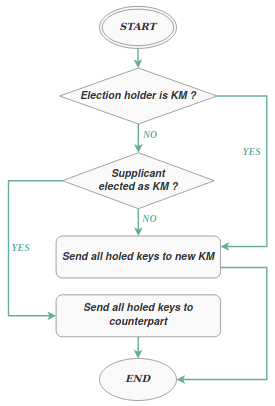
\includegraphics[scale=0.70]{figures/election_outcome.png}}
	\caption{Election outcome}
	\label{fig:election_outcome}
\end{figure}

\subsubsection{Election conflicts}

An eligible node, belonging to multiple groups, can participate in two election processes simultaneously. But if it gets elected in two distinct election process simultaneously, it shall assume the responsibilities of a KM where it’s more needed. For this purpose, a difference in the CEF score with the corresponding elected supplicant is measured. And where the difference is less significant, the node can decline the position to accept the other one. In other words, the choice goes to the group where the capability gap is wider in order to avoid under-performance issues. However, when a node is approved as a KM in a group’s election process, and as a supplicant in another, it would be accepting the KM position and declining the supplicant role. Nevertheless, if a node is simultaneously approved for supplicant in two elections, it can assume both as the supplicant role doesn’t have consequent heavy assignments.

For the following detailed example, we introduce the distance measurement:

\begin{equation}\label{eq5}
	d\left(n_1, n_2\right)  = e_k \; .\; \left( w_s s_k + w_n n_k +  w_p p_k \right)
\end{equation}

where
\begin{math}
	\left\{
	\begin{array}{l}
		c_k: capacity\; score\; of\; a\; node\; u_k\\
		w_s: storage\; capacity\; weight\\
		w_n: networking\; capacity\; weight
	\end{array}
	\right.
\end{math}\\

Let $n_i$ a technically capable node belonging to the groups $G_1$ and $G_2$, with both groups having an ongoing election process each. Let ${n_i}^1$ and ${n_i}^2$ also technically capable nodes belonging to $G_1$ and $G_2$ respectively. If parameter elected for $n_i$ is off, then it can broadcast its CEF score within the context of both groups as a potential candidate. If it receives an approval for the KM in a $G_1$ related election with ${n_i}^1$ as supplicant, it also receives approval as KM in the $G_2$ related election process with ${n_i}^2$ as supplicant, an arbitration should take place. Since the election is based on the CEF score, $n_i$ will measure the differences $d_1$ and $d_2$ with the node ${n_i}^1$ and ${n_i}^2$ respectively. $n_i$ will assume the charge of KM for the group related to the corresponding node with $m = max\left(d_1,\; d_2\right)$. Hence, it will decline the election approval for the other group, letting its corresponding deputy take over.

Fig.~\ref{fig:election_conflicts} illustrates the participation of the blue node in two separate elections with in the context of two different groups. The figure demonstrates how to proceed in case the blue node was elected as either KM or supplicant in both elections simultaneously. Table~\ref{tab:election_conflicts} sums the three cases up.

\begin{figure}
	\centering
	\begin{subfigure}[htbp]{0.3\textwidth}
		\centering
		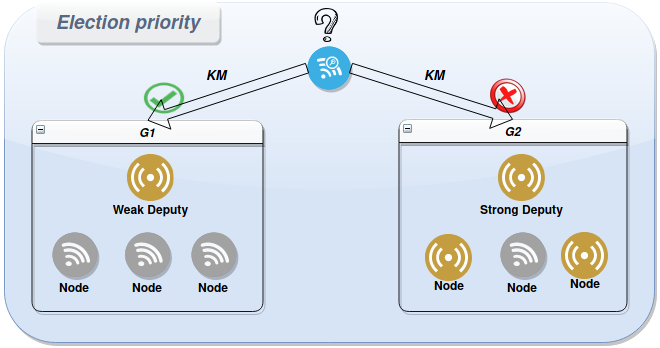
\includegraphics[scale=0.20]{figures/election2.png}
		\caption{Case 1}
		\label{fig:case1}
	\end{subfigure}
	\vfill
	\begin{subfigure}[htbp]{0.3\textwidth}
		\centering
		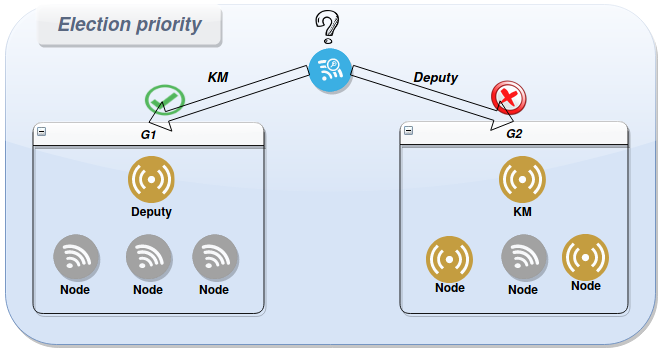
\includegraphics[scale=0.20]{figures/election3.png}
		\caption{Case 2}
		\label{fig:case2}
	\end{subfigure}
	\vfill
	\begin{subfigure}[htbp]{0.3\textwidth}
		\centering
		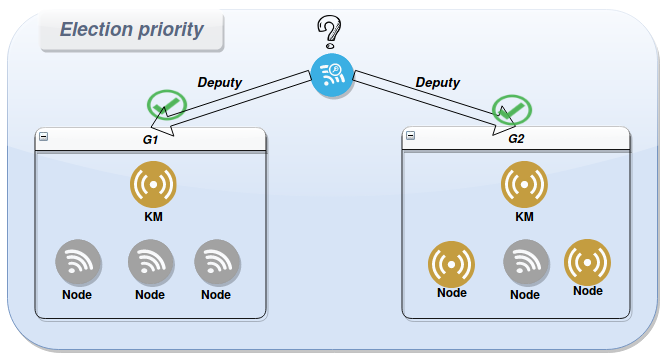
\includegraphics[scale=0.20]{figures/election4.png}
		\caption{Case 3}
		\label{fig:case3}
	\end{subfigure}
	\caption{Election conflicts}
	\label{fig:election_conflicts}
\end{figure}

\begin{table}[htbp]
	\caption{Election conflicts}
	\begin{center}
		\begin{tabular}{|c|c|c|c|}
			\hline
			\multicolumn{2}{|c|}{}&\multicolumn{2}{|c|}{\textbf{$G_1$ related election}} \\
			\cline{3-4} 
			\multicolumn{2}{|c|}{}& \textbf{\textit{Key Manager}}& \textbf{\textit{Supplicant}} \\
			\hline
			\textbf{$G_2$ related election}& \textbf{Key Manager}& verboten & verboten\\
			\cline{2-4}%\hline
			\textbf{$G_2$ related election}& \textbf{Supplicant} & verboten & allowed\\
			\hline
		\end{tabular}
		\label{tab:election_conflicts}
	\end{center}
\end{table}

\subsection{Failure recovery process}

There are three situations which could be qualified as failures requiring the instigation of a recovering process. In the first one, the KM is somehow unavailable, due to some flooding or a technical breakdown. The second situation concerns an attack leading to the compromise of the KM. And the last one is when a node is overworked and willing to hand over its responsibilities.

\begin{figure}[htbp]
	\centerline{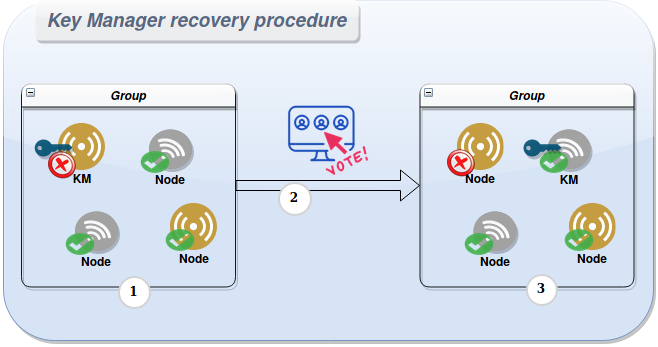
\includegraphics[scale=0.50]{figures/recovery.png}}
	\caption{Key Manager recovery routine}
	\label{fig:km_recovery}
\end{figure}

Starting with the first situation, the KM might be subject to overworking due to the important networking and processing overhead it has to bare. This could also be caused by veiled activities. Unless it has specific procedures to curb this burden, it obviously makes it vulnerable against breakdown. When the unwanted occurs, it’s first detected by the deputy KM, thanks to the regular check over procedure. Since the active KM will be unable to answer its deputy’s requests, this will let the latter know it’s technically down. From here, the supplicant broadcasts a claimer message to the group announcing that it’s taking over the leadership of the group. The former KM is excluded from the broadcast though. Then it starts a rekeying operation of the group. An finally, it calls for a new election to redefine who is the KM and his deputy on solid basis. We actually have no idea whether the breakdown is due to technical dysfunction or malicious attack such as DDoS. It could even be compromised by a malware, which prevents the reply upon check over to make it look like a normal breakdown. Keeping the former KM in the loop is exactly taking the risk of having a potential Trojan horse inside its network, without bothering taking any precautions. This significantly increases the resilience of the protocol.

\begin{figure}[htbp]
	\centerline{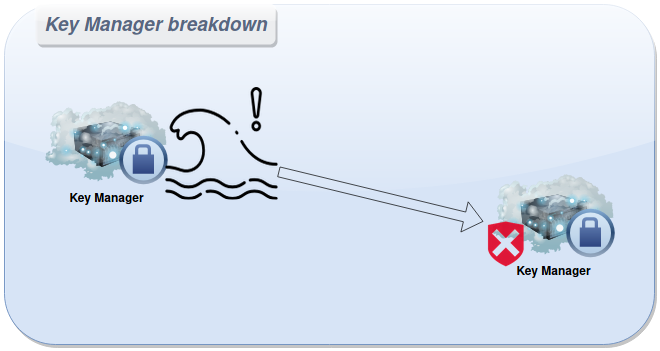
\includegraphics[scale=0.50]{figures/flooding.png}}
	\caption{Key Manager breakdown}
	\label{fig:km_breakdown}
\end{figure}

For the second situation, either we assume that we have a security entity (SE) physically separate from the KM (an IDS for example). It’s this component that guarantees the detection of eventual cyber attacks, and therefore, the instigation of the recovery process. Or, when in place, we can use the supplicant as a controller to detect the compromise, and so launch the recovery process. In the first case, we don’t consider the detection phase since it’s totally handled by the SE. But once the dysfunction is detected, the SE report directly to the KM deputy. In the second case, it’s the deputy KM that detects the compromise of its leader. The scenario would start with the supplicant receiving an inaccurate reply from the KM, upon a regular check over request. The inaccurate reply is basically a wrong answer to the deputy’s challenge. In both cases, the latter broadcasts then a disclaimer message to the concerned group fellows announcing that he is the new KM, while excluding the former one from the broadcast. It starts a rekeying operation after that of the group, since here we know for sure we have a node (the former KM) to evict. And finally, it calls for elections to settle a new appropriate KM, or at least fill in the vacant position of the supplicant.

\begin{figure}[htbp]
	\centerline{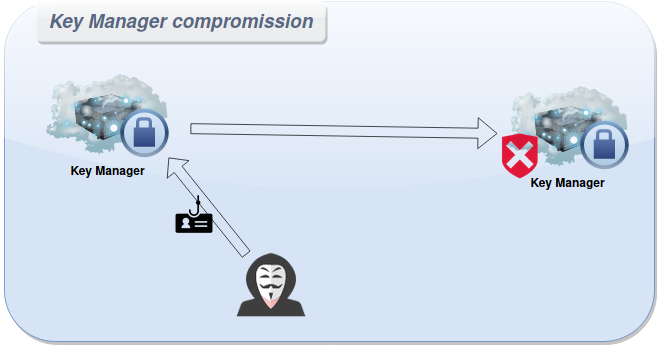
\includegraphics[scale=0.50]{figures/compromission.png}}
	\caption{Key Manager compromise}
	\label{fig:km_compromission}
\end{figure}

In this last situation, the KM isn’t necessarily suffering from any particular malfunctioning. For several reasons, it may choose to hand over its responsibilities to another node. It actually foresees some situation where, for application reasons, the KM will have additional expensive tasks to handle besides the Key Management ones, exceeding its capacities. The step off cause might simply be the KM leaving the group too as part of the application. Instead of forwarding the task to the deputy, it first calls for anticipated election in which it would not be a candidate. The election will output a newly KM . Only then, the desisting KM hand over the role to the latter.
%
%[TODO dig and develop the 3rd case]

\begin{figure}[htbp]
	\centerline{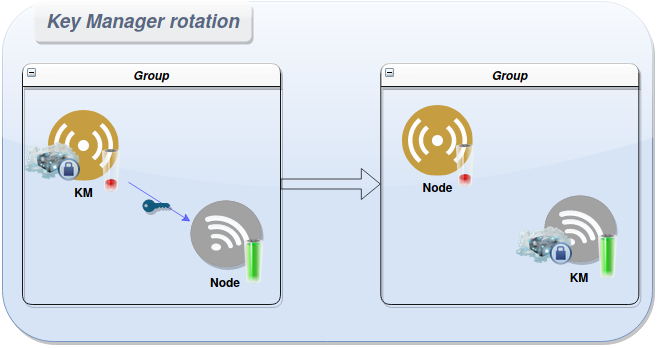
\includegraphics[scale=0.50]{figures/rotation.png}}
	\caption{Key Manager turnover}
	\label{fig:km_turnover}
\end{figure}

The scheme, as explained, introduces a supplicant which monitors the active KM and ready to take over in need, while actually allowing any node to be the KM itself. This alongside the performance optimisation introduced for new key sharing, are made up to address the issue of \textit{\textbf{single point of charge}}. With in the same progress line, the capability-based election process concatenated with the failure recovering processes, their conditions and the supplicant’s monitoring are actually made up to address the issue of \textit{\textbf{single point of trust}}. This way, the overall election-based scheme solves the issue of \textit{\textbf{single point of failure}}, by locking on the different reasons which led to this problem in the first place, as well as its unexpected consequences.

\begin{figure}[htbp]
	\centerline{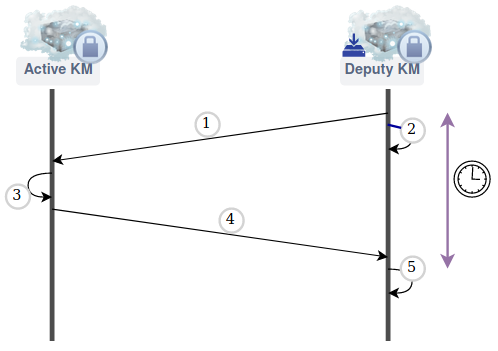
\includegraphics[scale=0.50]{figures/check_over.png}}
	\caption{Check over message exchange}
	\label{fig:double_check_exchange}
\end{figure}

Fig.~\ref{fig:double_check_exchange} illustrates the message exchange for a routine check over procedure. Above labeled steps correspond to:

\quad(1) Challenge request

\quad(2) Set timer on

\quad(3) Answer computation

\quad(4) Challenge reply

\quad(5) Set timer off + Challenge validation

The challenge validation implies both, a correct answer to the request and a response time within the set timeout.

An alternative routine would be the supplicant listening to the active KM, whereas the latter sends regular messages to its deputy announcing it’s still up. For integrity consolidation these messages have to be cryptographically signed. This pulse-check routine reduces the networking overhead by a factor of two. Although from a security point of view, it’s much less reliable than the check-over routine previously described.

In order to combine advantages of both routines, we define a hybrid solution, where regular checks are performed every time lapse, referred as $\Delta$t. These checks are mostly simple pulse-checks. But every certain number of time slots $\Delta$t, referred as $nc$, we perform the double check-over routine.

\begin{figure}[htbp]
	\centerline{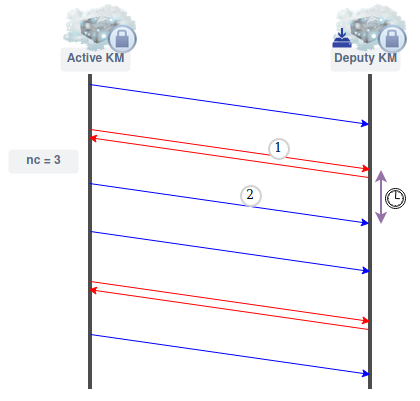
\includegraphics[scale=0.50]{figures/check_routine.png}}
	\caption{Check Over routine}
	\label{fig:check_over_routine}
\end{figure}

This way, we ensure availability and integrity of the KM, while significantly reducing the networking and processing overhead for both parties. $\Delta$t and nc are settable and configurable parameters, since depending on the actual use case, the balance between performance and security might flip to either side. If we want to keep only the first routine, one can just set $nc$ to $nc = null$. The bigger $\Delta$t is, the smaller the networking overhead is. Fig.~\ref{fig:check_over_routine} illustrates this hybrid solution, with:

\quad(1) Double-way check-over routine

\quad(2) One-way check-over routine

\subsection{Security analysis}

The CEF score is intentionally designed to be an average value totally blending regarding the input values. It’s actually more secure if the CEF score doesn’t leak any data about a node’s real capabilities in terms of networking, storage and processing. Knowledge of some physical properties of a device can be used to mount cryptanalytical side-channel attacks. During an election process, any group member node $u$ shall be able to capture CEF scores of other fellow nodes. But it won’t need these information as long as it’s a fellow member of the group and holds required keys to decipher transiting communications. When $u$ leaves the group or gets evicted, the MGKM protocol relies on the group rekeying in order to guarantee forward secrecy. The recently leaving (or evicted) node $u$ can seek to decipher group’s communications based on its previously acquired knowledge on communicating entities. This way, forward secrecy is put at risk. This also applies for a recently joining node $v$. During the first election process after its join, different nodes will be broadcasting their respective CEF scores, which express their respective physical capacities. The node $v$ might then use these acquired scores to carry out side-channel cryptanalysis attacks on encrypted messages collected before its join. This way, backward secrecy is put at risk. Since the CEF’s output is a single dark value, it will therefore prevent these category of cryptanalysis attacks. Hence, our solution maintains forward and backward secrecy properties.

When a node $u$ acting as KM is compromised and evicted, the supplicant immediately takes over the group leadership and rekeys the group, while excluding the former KM from this rekeying process. Only afterwards it calls for an election and kicks the election process off. Messages related to the election which would take place will be encrypted using a newly generated group key. By applying the forward secrecy principle guaranteed by the rekeying process, the former compromised KM will hence be unable to decipher them. The group’s communications are then secure.

Another security issue had to be considered when designing the check over process. As previously hinted, the simple check over routine utilizes cryptographic message signature only as a security measure to authenticate the KM. However, the double check over routine utilizes challenge-response authentication which can be (but not necessarily) coupled with cryptographic message signature as security measures. The latter is obviously more secure, but less efficient. The combination of how all of this will be implemented is left to the eventual R\&D engineer who might take over the protocol. What actually interests us here is the foreseen security cradle put in place for the overall check over process. Now both considered measures have their own advantages and drawbacks, with the challenge-response authentication slightly safer. Nevertheless, none of both can be taken for granted. On one hand, new attacks on both keep surfacing constantly. On the other hand, both are hardened and enhanced continuously. Besides, these measures themselves bring their own parameters and vulnerabilities. As seen in Section~\ref{subsec:cryptography}, the choice of message authentication codes and signature algorithms can have a huge security impact. In the same line, different challenge-response protocols for different situations exist. The engineer implementing the process knows his own use case and security risks. Therefore, he knows better which combination of all this fits best.

In short, the check over process intentionally embeds two different and combinable security measures. The objective is to offer a maximum of options for different security situations.

\subsection{Discussion}

The following discussion brings nothing new in term if technical specification. But since this a fundamental research work, it's more destined, but not only, to any eventual engineer who might be implementing the solution. This paragraph actually tries to give a glimpse on how practical the solution is and what kind of asset and disadvantage the above technical description can have on the implemented system.

\subsubsection{Flexibility and adaptability}

The main drawback of this scheme, is the networking overhead that comes with. Despite the suggested optimisations, we still have a high number of required messages to undergo related procedures and processes. In order to get over this lack, the scheme should be designed in a flexible way.

For the protocol’s operational mode, the CH rotation has to be implemented carefully, and sometimes, even set as optional. This could be very well relevant to some applications where the KM’s choice is static and permanent (eg. Cloud server). In this case, all message exchange relevant to CH rotation is probably useless and a waste of bandwidth and energy.

Besides, the supplicant role should be optional. We can’t be always sure whether we will dispose of enough qualified candidates for both roles. And sometimes, the infrastructure could designed in a way that one particular component is intended to be the KM for his group. In which case, the engineers building the infrastructure could have foreseen alternative measures to sort out any failure in the KM. Furthermore, the supplicant plays also a security role as it monitors the KM’s availability. Depending on the global infrastructure and the KM’s ecosystem, this role could be obsolete since there is some other component doing it. In the same line of thought, this so-called powerful KM could foreseen by its implementing engineers to cover more than one group. Thereby, the mutual exclusion in elections should be optional as well, in particular, disabled. In this direction, it seems at first we’re heading back towards the original centralised KM scheme. Nevertheless, the idea of the election-based scheme is to tackle the issue of single point of failure. But the last call is left to the engineer implementing the protocol, so that it offers the protection it claim when necessary. Besides, the scheme introduces itself as a compromise between centralised (unique KM) and fully decentralised (Blockchain) schemes. This way, among n groups, we can have one or some of them managed by one capable KM, technically just by disabling an option, while the rest of the groups dispose of their own elected KM. So here the scheme doesn’t cover the whole infrastructure, but it’s used right where it’s needed to tackle the central problem previously defined. And this is particularly useful for heterogeneous networks. This also facilitates migration from centralised solution to this one.

As for the election process, the elected parameter blocking mode has to be implemented in a way it can only be enabled manually. The feature should basically be optional. This feature is useful in some cases where we might have some very battery-weak devices. Despite the set eligibility threshold, just the computation of the CEF and the preliminaries could be, for some devices, enough for the battery to be rolled out. Nevertheless, this option isn’t pertinent for all IoT use cases. And since it brings in restrictive measures for concerned nodes, then it should definitely be configurable only manually depending on the application.

The eligibility definitely cannot be stiff. In order to improve the scalability and adaptability of the protocol regarding heterogeneity, CEF threshold has to be optional and configurable as well. Depending on the application, we can have very different scales of devices power. Thereby, the very definition of a powerful node would change. Hence, we shall be able able to lower down our standards, even sinking it til 0 if necessary. On the other side, we could be willing to top it up, if the engineer implementing is sure about the robustness of his devices and his need for a very reliable KM. This CEF feature might also be left open for more input criteria (or less) depending on the use case. Nevertheless, it has always to remain as static as possible and least possible dependant on dynamic inputs. The latter actually can increase the turn over rate for the score’s update, and so, an increase in the computation overhead.

Concerning the overall architecture of the protocol, it actually relies on one KM assigned to one group basically. This should be extensible for other layers of the infrastructure, such as having one KM per service or per subgroup. Such architectures and configurations have to be thought over and studied in depth, in order to conclude on their utility, efficiency and feasibility.

\subsubsection{Inter-group communications management}

Another approach would be based on a double layer election. The first defined KM election would be regarded as a local group election. We introduce a federal election which takes place between different local KMs, in order to elect a federal KM. The latter would then assume a double role, (i) managing his own group’s keys and (ii) handling inter-group related keys. The local KMs are the only eligible candidates, and in the same time, the only voters. The rest of the election process goes the same as for the local one. This approach has the advantage that it bypasses all possible management conflict which might pop up according to the first suggestion. Typically, this might occur when the rekeying process concerns a node belonging to different groups sharing the same service. Hereby, more than one KM is supposed to handle the service keys, making a part of the process redundant between different concerned KMs. A drawback however shines when it comes to profitability. This approach is less scalable and efficient than the previous one.

\section{Simulations and results}
\label{sec:simulations_results}

A simulator of the MGKMP was developed as part of the PhD thesis \cite{kandi_lightweight_nodate} anterior to this work. After studying the code source, the program was actually implemented to simulate the protocol's rekeying process and sub-grouping algorithms. Thus it's not fit for this use case. Working on this simulator to adapt it was considered indeed. However, this would have taken much more time than implementing a new one dedicated to the ongoing situation. The second solution was picked, because the simulation phase came at a time when the conference deadline for paper submission was closing in.

\subsection{Simulator implementation}

Two simulators were implemented with different levels of success. The programming language of choice for both is \emph{Python3}. The first is much more complete and realistic, but has a lot of bugs. The second one is simpler, but still produced some decent results. The development approach adopted is object-oriented.

First of all, I thought of implementing a simulator, which will simulate the whole MGKMP architecture. In other terms, the simulator actually implements possible entities such as nodes, KM, groups and subgroups. The communication between different nodes takes place via network sockets. The simulator uses the \emph{select} function from the \emph{Socket API} to handle connections for every node. The simulated algorithms mainly include those related to the election-based scheme, ie. the election and  check-over processes. The messages exchanged were also implemented to be encrypted, to provide the most realistic environment possible. This simulator is pretty sophisticated, so its implementation requires several functions management and consequent debugging. Due to time constraints, it couldn't be finished. So I switched to a similar simulator, but with some features cut off.

The second simulator doesn't emulate the MGKMP architecture entirely. It only considers one group with several nodes, two of which are KM and Supplicant respectively. It does implement a messaging structure. But communications and encryption are actually abstracted, they go through the \emph{Simulator} object. The latter acts as the orchestrator running the show. It coordinates exchanges between different nodes and calls election related algorithms when needed. So this simulator is only good enough to emulate the algorithmic behavior of the developed solution, as well as the influence of different parameters variation.

The \emph{Node} object has two different categories of attributes. First, it has physical capabilities such as radio range and processing capacity. Those values are random, attributed at the simulation's start and remain unchanged all along. They are different for every node. Second, it also has volatile attributes which tend to evolve overtime, such as the percentage of processor in use and residual energy. These attributes start with the same values for all nodes. For example, the starting residual energy for all nodes is set to $re = 1000$, which is the maximum. Then it decreases overtime according to the simulation's events at a different pace for each node. Capabilities values aren't realistic, but rather based on a scale in such a way to have credible comparisons.

In order to generate results, the main program is implemented in \emph{results.py}. It starts a simulation according to given parameters ($\Delta t$, $nc$, $rt$ \ldots). Then, it stimulates different processes such as election or check-over routines. On every new event, it takes snaps, which mean it gathers information about all nodes and simulation status and stores them in a file. Based on these files, the program can generate graphics using the \emph{matplotlib} library.

\subsection{Simulation results}

In the following examples, we assume that a node which was previously elected KM cannot be re-elected. Thus to measure the influence of KM turnover on the overall organization.

The simulator initiates 8 nodes at first, none of which is KM nor Supplicant. These nodes are attributed random physical capacities as mentioned, so they can compute their initial CEF score respectively. The initial status is saved to \emph{snap00}.

In the first scenario (see Appendix~\ref{app:example1}), the simulator instigates a first election, during which \emph{Node 6} is elected KM and \emph{Node 7} is elected Supplicant. Then it instigates a second election, during which \emph{Node 7} is elected KM and \emph{Node 1} is elected Supplicant. Fig.~\ref{fig:sim_exmp1} illustrates the energy and CEF score evolution of \emph{Node 7}. Between $t = 0$ and $t = 3$, the node acted as Supplicant and its energy is hence decreasing. The second election took place between $t = 3$ and $t = 6$, after which \emph{Node 7} became KM. What the figure illustrates, is that during the same time lapse ($\Delta t= 3$), the election process if far more exhausting than the check-over.

\begin{figure}[htbp]
	\centerline{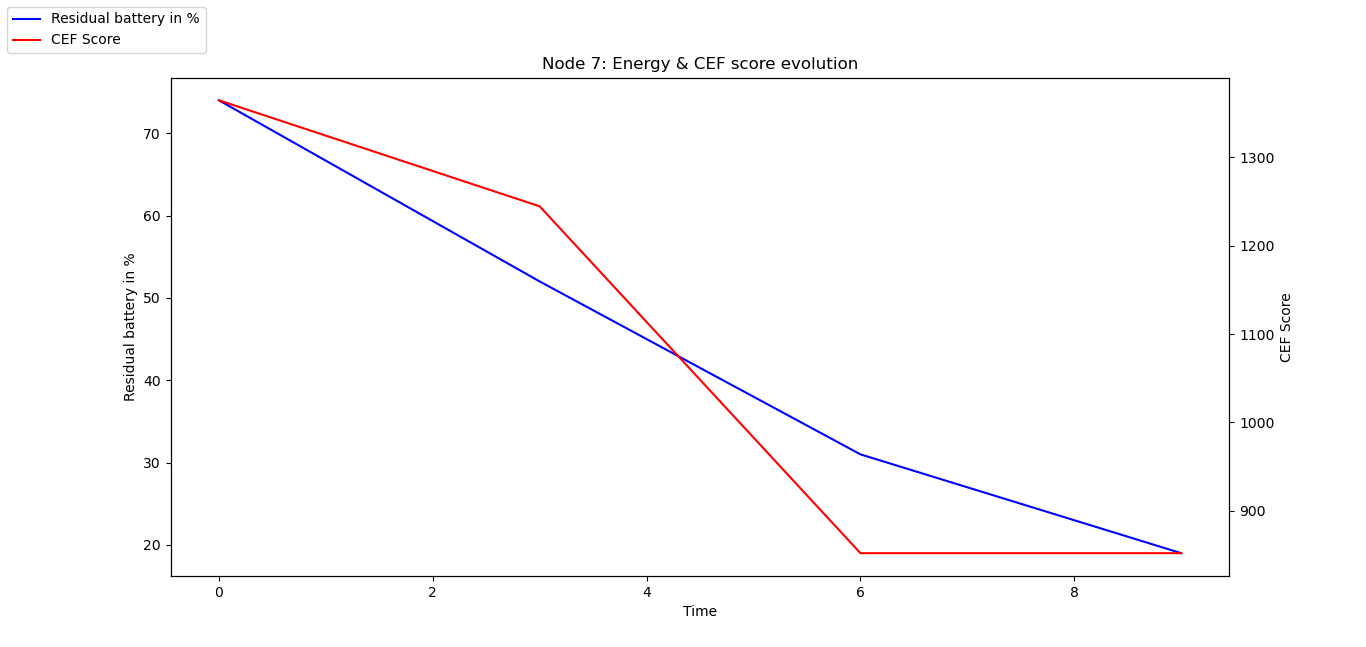
\includegraphics[scale=0.35]{figures/simulation/energy_cef_evolution.png}}
	\caption{Node 7: Energy \& CEF score evolution}
	\label{fig:sim_exmp1}
\end{figure}

In as a second scenario, the simulation tries to assess the influence of $nc$ value on the solution. The election process is a random event. Hence, I concentrated more on the check over process, since I have more control on its occurrence frequency.

Let's assume that a check process, whether simple or double, is an atomic operation. We fix the time gap between two consecutive checks to $\Delta t = 2$, and the simulation duration is fixed on 36 time units. The simulation consists in running the check-over routine over the simulation duration straight with different values of $nc$, and measure the energy consumption for both, the KM and its deputy. The $nc$ value range goes from 1 to 30. Intuitively, a decrease in consumed energy during the simulation is expected as $nc$ is increased, since a one-way check consumes less than a double one. From an energy perspective, we tend to increase this value. From a security perspective, we tend to decrease it. The objective is to find a satisfactory compromise.

\begin{figure}[htbp]
	\centerline{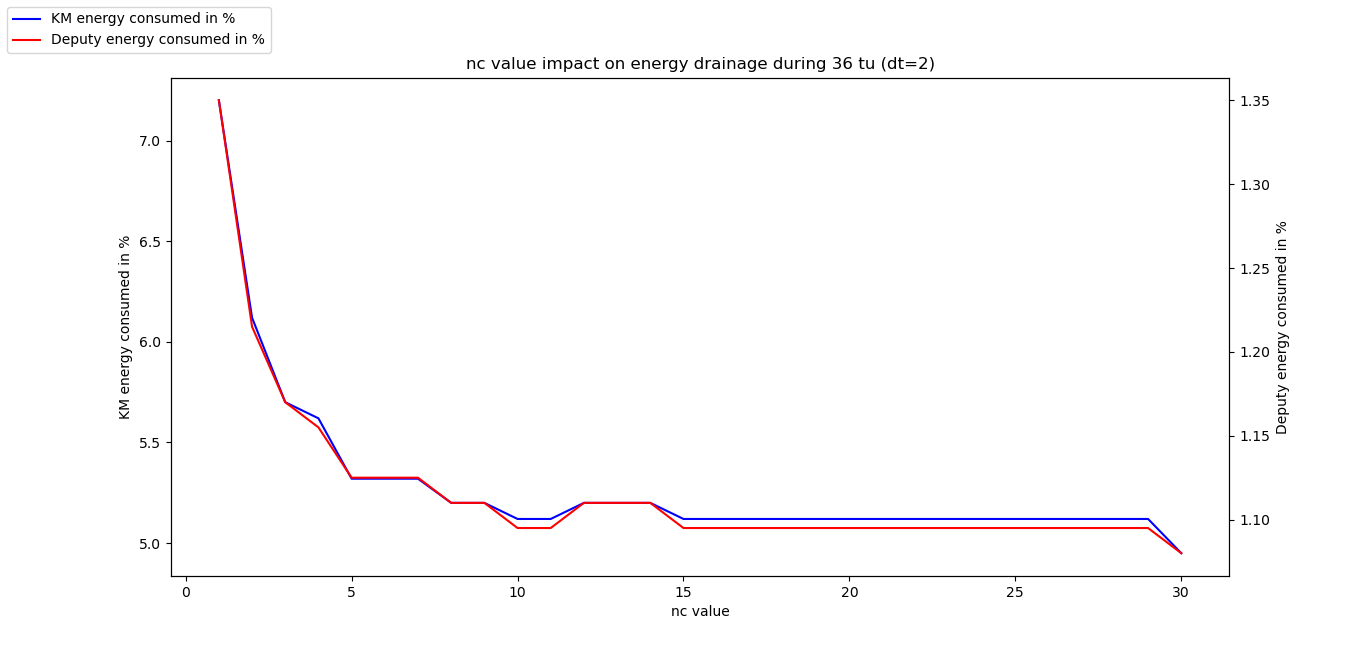
\includegraphics[scale=0.35]{figures/simulation/nc_energy.png}}
	\caption{Variation of energy drainage according to $nc$ value}
	\label{fig:sim_nc_impact}
\end{figure}

Fig.~\ref{fig:sim_nc_impact} shows that this compromise can be quickly found, and it’s valid for our two measured entities. The gain in energy grows pretty fast as we increase $nc$ value between $nc=5$ and $nc=10$. Therefore, our algorithm is able to reach good energy performances, while keeping a certain security level ensuring the KM’s integrity. There is a slight illogical increase in energy between $\Delta t = 12$ and $\Delta t = 14$ though. The reason isn't clear, but it could be explained by the simulator's random behavior.

It's \textbf{\textit{very important}} to note that interpretations rely only on figures shape, regardless of the scales or values. As said before, the program simulates the algorithmic behavior of protocol. So we know that in a more realistic experiment, we would still get the same figure's shape, but the output values can be different. For example, Fig.~\ref{fig:sim_nc_impact} shows that between $nc=1$ and $nc=5$, energy drainage dropped by approximately 1.9\%. It's this kind of value which is irrelevant, because physical capabilities are randomly attributed and disconnected with the physical realm.

\section{Future work}

If I pick up where I last left off, it is clear that simulations and experiments need to be pushed way further. First, simulations remain in their early stages. More tests should be carried out using a more sophisticated and realistic simulator. Second, real laboratory experimentation has to be carried out to observe the divergence between simulations and experiments, and eventually address the gap. The simulator itself isn't fully implemented. From a functional point of view, many features are poorly developed. For instance, a node can have a negative battery value, absolutely mind blowing. That's because until this point, these features aren't required to retrieve the needed measures. But as the simulations get more advanced, it's better to have something more complete. From a structural point of view, it's also better to make the simulations more realistic, regarding how nodes are organized and communicating. This actually goes back to finishing the second simulator which didn't work out in this internship.

Another task to look closer concerns the algorithms complexity. In this chapter, no such mathematical study was made, and yet it's important to assess. It was shown through simulations that election and check-over algorithms don't have the same energy consumption for example. A more more profound algorithmic study can reveal the exact difference, and eventually contribute in the complexity optimization.

Moreover, all issues described in Chapter~\ref{chap:mgkmp} need to be treated the same way as the Key Manager. In particular, the work on the CEF score done in this internship can be inter-crossed with the subrouping sequences (Section~\ref{subsec:subgroups}) and $mc$ values.